\documentclass[12pt]{article}
\usepackage{graphics, graphicx, cite, fancybox, setspace}
\usepackage{amsfonts, amssymb, amsmath, latexsym, epic, eepic, url}
\usepackage{algorithm}
\usepackage{algorithmic}
\usepackage[letterpaper, left=1in, right=1in, top=1in, bottom=1in]{geometry}
\usepackage{times}
\usepackage[parfill]{parskip}

\begin{document}

\title{Introduction to Parallel Computer Architecture \\
Numerical Integration using the Trapezoidal Rule}
\author{Instructor: Prof. Naga Kandasamy \\ ECE Department, Drexel University}
\maketitle %
\date{}

Given a function $f(x)$ and end points $a$ and $b$, where $a < b$, we wish to estimate the area under this curve; that is, we wish to determine $\int_{a}^{b} f(x)\, \mathrm{d}x$.

\begin{figure}[!h]
\centering
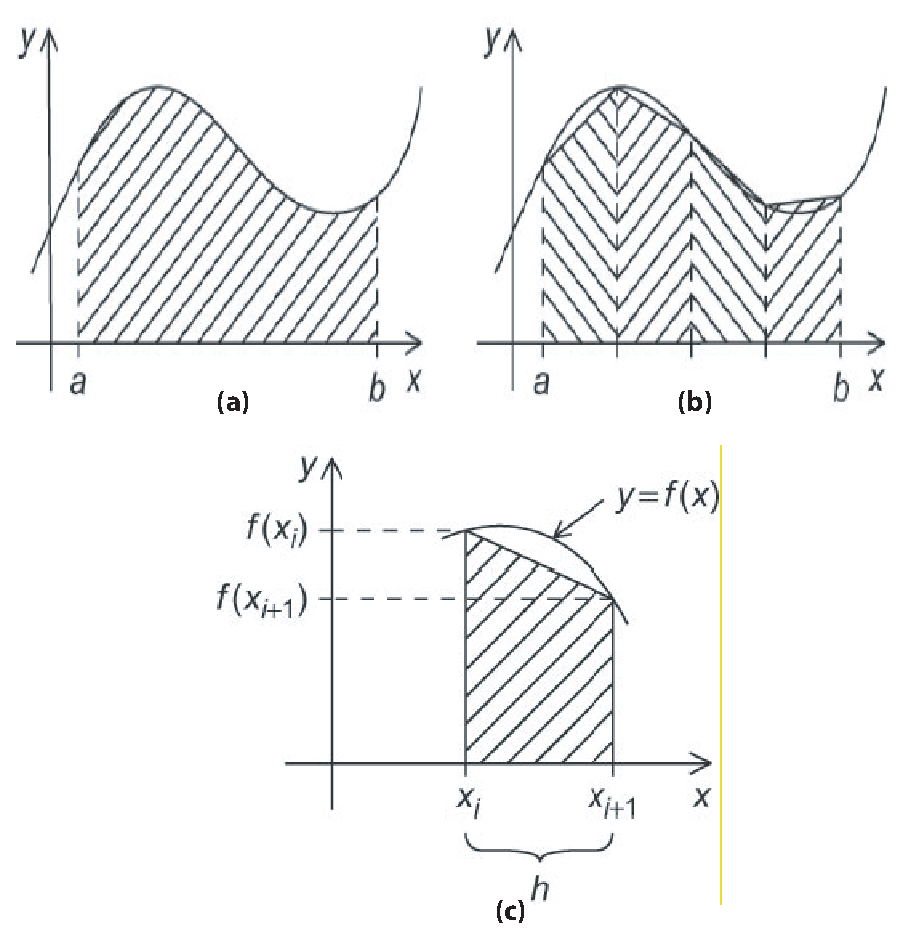
\includegraphics[width=3in]{trap}
\caption{Illustration of the trapezoidal rule: (a) area to be estimated; (b) approximate area using trapezoids; and (c) area under one trapezoid.} \vspace{-6pt}
\label{fig:trap}
\end{figure}

The area between the graph of $f(x)$, the vertical lines $x = a$ and $x = b$, and the $x$-axis can be estimated as shown in Fig.~\ref{fig:trap} (b) by dividing the interval $[a, b]$ into $n$ subintervals and approximating the area over each subinterval by the area of a trapezoid. Fig.~\ref{fig:trap}(c) shows one such trapezoid where the base of the trapezoid is the subinterval, its vertical sides are the vertical lines through the endpoints of the subinterval, and the fourth side is the secant line joining the points where the vertical lines cross the graph. If the endpoints of the subinterval are $x_i$ and $x_{i+1}$, then the length of the subinterval is $h = x_{i + 1} - x_i$, and if the lengths of the two vertical segments are $f(x_i)$ and $f(x_{i + 1})$, then the area of a single trapezoid is $\frac{h}{2}[f(x_i) + f(x_{i+1})]$. If each subinterval has the same length then $h = (b - a)/n$. Also, if we call the leftmost endpoint $x_0$ and the rightmost endpoint $x_n$, we have
\begin{equation*}
x_0 = a, x_1 = a + h, x_2 = a + 2h, \ldots, x_{n-1} = a + (n-1)h, x_n = b,
\end{equation*}
and our approximation of the total area under the curve will be
\begin{equation*}
\int_{a}^{b} f(x)\, \mathrm{d}x = h[f(x_0)/2 + f(x_1) + f(x_2) + \cdots + f(x_{n-1}) + f(x_n)/2].
\end{equation*}

Thus, the pseudo-code for a serial algorithm might look something like the following.
\begin{algorithm}[!h]
\begin{algorithmic}[1]
	\STATE \textbf{procedure} TRAP($a$, $b$, $n$)
    \STATE $h$ := $(b - a)/n$;
    \STATE $sum$ := $(f(a) + f(b))/2.0$;
    \FOR{$i$ := 1 to $n-1$ step 1}
        \STATE $x_i$ := $a + i \times h$;
        \STATE $sum$ := $sum$ + $f(x_i)$;
    \ENDFOR
    \STATE $sum$ := $h \times sum$;
\end{algorithmic}
\end{algorithm}

\end{document}
